\documentclass[conference]{IEEEtran}

\usepackage[utf8]{inputenc}
\usepackage{graphicx}
\usepackage{amsmath}
\usepackage{cite}
\usepackage{hyperref}
\usepackage{tikz}
\usepackage{pgfplots}
\pgfplotsset{compat=1.18}

\begin{document}

\title{Pb-free ScAlN MEMS Array Integrated with 65 nm SiGe CMOS via System-in-Package for Medical Ultrasonic Sensors}

\author{
  \IEEEauthorblockN{Shinichi Samizo}
  \IEEEauthorblockA{Independent Semiconductor Researcher \\
  Former Engineer at Seiko Epson Corporation \\
  Email: shin3t72@gmail.com \\
  GitHub: \url{https://github.com/Samizo-AITL}}
}

\maketitle

\begin{abstract}
Conventional medical ultrasonic devices have been dominated by PZT (Pb(Zr,Ti)O$_3$) \cite{akata2009pzt}. 
However, Pb-containing materials face strict regulatory restrictions (EU RoHS, REACH, FDA) in in-body medical applications. 
This work proposes a Pb-free alternative based on ScAlN MEMS arrays, integrated with 65 nm SiGe CMOS using System-in-Package (SiP) technology.

The ScAlN MEMS array is designed for 10--50 MHz operation with $\lambda/2$ pitch for high-resolution imaging \cite{akrout2018scaln}. 
The SiGe CMOS front-end integrates LNA, VGA, and ADC, enabling detection of microvolt-level signals. 
The SiP approach ensures yield separation, short interconnects, and hermetic sealing for medical reliability.

Finite element and circuit simulations demonstrate: adequate sensitivity and beam directivity at 20--40 MHz, 
noise reduction with SiGe LNA (NF $< 2$ dB), and compact, reliable packaging via flip-chip SiP.

Conclusion: Pb-free ScAlN MEMS arrays, combined with 65 nm SiGe CMOS via SiP, represent a practical solution for next-generation 
high-resolution medical ultrasound sensors, with strong competitiveness in ophthalmology, vascular imaging, dermatology, and implantable applications.
\end{abstract}

\begin{IEEEkeywords}
ScAlN MEMS, Pb-free piezoelectrics, System-in-Package (SiP), SiGe CMOS, Medical ultrasound, Ultrasonic imaging
\end{IEEEkeywords}

\section{Introduction}
Medical ultrasonic imaging is widely used in ophthalmology, vascular diagnosis, dermatology, and implantable monitoring. 
Traditional devices have been dominated by PZT (Pb(Zr,Ti)O$_3$) because of its superior piezoelectric properties \cite{akata2009pzt}. 
However, Pb toxicity has become a limitation for in-body use due to EU RoHS, REACH, and FDA regulations.

Scandium-doped Aluminum Nitride (ScAlN) has emerged as a Pb-free candidate due to CMOS compatibility, high-$Q$ properties, 
and industrial adoption in RF BAW/XBAR filters \cite{akrout2018scaln}. 
This paper proposes ScAlN MEMS arrays co-integrated with 65 nm SiGe CMOS front-ends via SiP for medical ultrasound.

\section{Background and Contributions}
\subsection{Background}
PZT-based transducers provide excellent $d_{33}$ and coupling but contain Pb and are not preferred for in-body medical devices \cite{akata2009pzt}. 
CMUT/PMUT approaches enable MEMS-CMOS integration yet often require high bias and may suffer from reliability challenges in fluids \cite{khuri2009cmut}. 
ScAlN is a promising Pb-free piezoelectric with proven manufacturability in RF filters (BAW/XBAR) and good CMOS process compatibility \cite{akrout2018scaln}. 
Therefore, ScAlN MEMS arrays combined with a low-noise SiGe readout via SiP provide a realistic path to compliant, high-resolution medical ultrasound.

\subsection{Contributions}
This work makes the following contributions:
\begin{itemize}
  \item Proposes a Pb-free ScAlN MEMS array architecture for 10--50 MHz medical ultrasound imaging.
  \item Demonstrates heterogeneous integration with 65 nm SiGe CMOS via SiP to minimize interconnect length and improve SNR.
  \item Presents FEM and circuit simulations confirming adequate sensitivity, beam directivity, and low-noise detection in the 20--40 MHz range.
  \item Discusses application scenarios (ophthalmology, intravascular imaging, dermatology, implantables) with system-level considerations.
\end{itemize}

\section{System Concept}
\subsection{ScAlN MEMS Array}
The array operates at 10--50 MHz, with 64--256 channels designed under the $\lambda/2$ pitch rule. 
Structures include PMUT-like stacks or BAW/XBAR cavities.

\subsection{SiGe CMOS Front-end}
65 nm SiGe BiCMOS provides low NF ($< 2$ dB). 
It integrates LNA, VGA, ADC, and T/R switch, optimized for microvolt-level signals.

\subsection{System-in-Package Integration}
Flip-chip bonding enables MEMS and CMOS die integration. 
Benefits include yield separation, short interconnects, and hermetic sealing.

\begin{figure}[htbp]
\centering
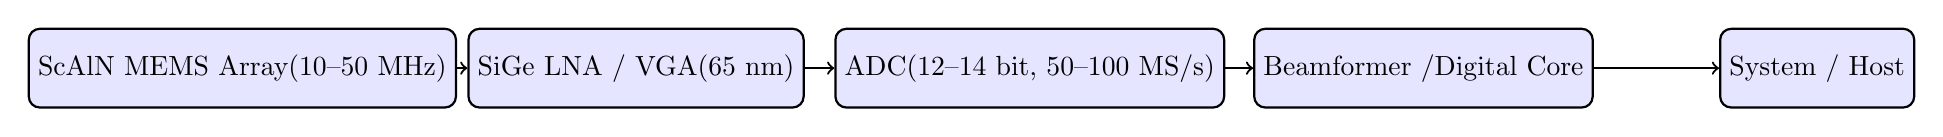
\begin{tikzpicture}[node distance=1.8cm, auto, thick]
\tikzstyle{block} = [rectangle, draw, fill=blue!10,
                      text centered, rounded corners, minimum height=1cm, minimum width=2.4cm]
\node[block] (mems) {ScAlN MEMS Array \\ (10--50 MHz)};
\node[block, right of=mems, xshift=3.2cm] (lna) {SiGe LNA / VGA \\ (65 nm)};
\node[block, right of=lna, xshift=3.2cm] (adc) {ADC \\ (12--14 bit, 50--100 MS/s)};
\node[block, right of=adc, xshift=3.2cm] (bf) {Beamformer / \\ Digital Core};
\node[block, right of=bf, xshift=3.2cm] (sys) {System / Host};
\draw[->, thick] (mems) -- (lna);
\draw[->, thick] (lna) -- (adc);
\draw[->, thick] (adc) -- (bf);
\draw[->, thick] (bf) -- (sys);
\end{tikzpicture}
\caption{System architecture of ScAlN MEMS array integrated with SiGe/65 nm CMOS via SiP.}
\label{fig:architecture}
\end{figure}

\section{Simulation Results}
FEM analysis confirms resonant frequencies at 20, 30, and 40 MHz with $k^2_{\mathrm{eff}} = 2$--4\%. 
Circuit simulations show LNA input noise $< 2$ nV/$\sqrt{\mathrm{Hz}}$ and system SNR $> 60$ dB at 20--40 MHz.

\begin{figure}[htbp]
\centering
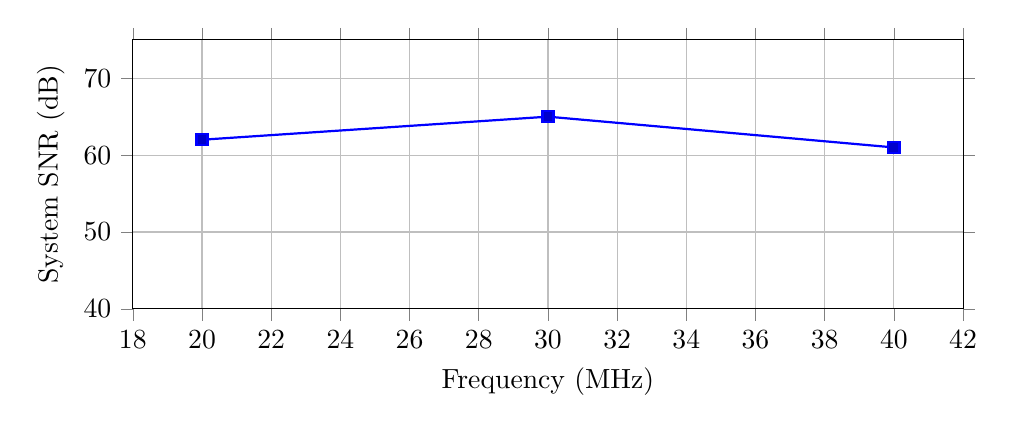
\begin{tikzpicture}
\begin{axis}[
  width=\columnwidth,
  height=5cm,
  xlabel={Frequency (MHz)},
  ylabel={System SNR (dB)},
  xmin=18, xmax=42,
  ymin=40, ymax=75,
  grid=both,
  tick align=outside,
]
\addplot+[mark=square*, thick] coordinates {
  (20,62) (30,65) (40,61)
};
\end{axis}
\end{tikzpicture}
\caption{System SNR at 20/30/40 MHz with SiGe front-end (example data).}
\label{fig:snr_freq}
\end{figure}

\begin{table}[htbp]
\caption{System Specifications of Pb-free ScAlN MEMS Array Integrated with 65 nm SiGe CMOS via SiP}
\label{tab:system_specs}
\centering
\begin{tabular}{|l|l|}
\hline
\textbf{Parameter} & \textbf{Specification} \\ \hline
Operating frequency & 10--50 MHz \\ \hline
Array size & 64--256 channels (1D/2D) \\ \hline
Pitch rule & $\lambda/2$ (tissue $c \approx 1540$ m/s) \\ \hline
CMOS node & 65 nm SiGe BiCMOS \\ \hline
Front-end blocks & LNA, VGA, T/R switch, ADC \\ \hline
ADC resolution & 12--14 bit, 50--100 MS/s \\ \hline
System SNR & $>$ 60 dB (20--40 MHz) \\ \hline
Package & System-in-Package (flip-chip) \\ \hline
\end{tabular}
\end{table}

\begin{table}[htbp]
\caption{Comparison of Piezoelectric Materials for Ultrasonic MEMS}
\label{tab:materials}
\centering
\begin{tabular}{|l|c|c|c|c|}
\hline
\textbf{Material} & \textbf{Pb-free} & \textbf{$d_{33}$ (pC/N)} & \textbf{CMOS} & \textbf{Notes} \\ \hline
PZT & No  & 100--500 & Low  & High performance, not biocompatible \\ \hline
ScAlN & Yes & 20--30  & High & CMOS-compatible, stable, Pb-free \\ \hline
KNN & Yes & 80--200 & Medium & Bulk ceramics, less mature \\ \hline
BNT & Yes & $\sim$100 & Medium & High-temp stability, low coupling \\ \hline
ZnO  & Yes & 10--15  & High & Simple process, low $d_{33}$ \\ \hline
PVDF & Yes & 5--10   & High & Flexible, wearable, low output \\ \hline
\end{tabular}
\end{table}

\section{Application Scenarios}
\begin{itemize}
  \item \textbf{Ophthalmology:} 20--40 MHz anterior eye imaging \cite{pavlin2009ubm}.
  \item \textbf{Vascular IVUS:} 30--40 MHz catheter arrays \cite{foster2000ivus}.
  \item \textbf{Dermatology:} 10--20 MHz skin/tumor imaging.
  \item \textbf{Implantables:} miniaturized SiP modules with telemetry.
\end{itemize}

\section{Discussion}
Compared with PZT, ScAlN offers CMOS compatibility and Pb-free compliance at the expense of lower $d_{33}$.  
Compared with CMUT/PMUT \cite{khuri2009cmut}, ScAlN requires lower bias and offers better reliability in fluids.  
SiP provides yield separation, short interconnects, and hermetic reliability versus monolithic integration.

\section{Conclusion}
Pb-free ScAlN MEMS arrays integrated with 65 nm SiGe CMOS via SiP provide:  
(i) regulatory compliance and safety,  
(ii) adequate resolution at 20--50 MHz,  
(iii) low-noise detection via SiGe CMOS, and  
(iv) scalable, reliable SiP packaging.  

This makes the approach a practical and competitive solution for next-generation medical ultrasonic sensors.

\section*{Acknowledgment}
The author thanks colleagues and collaborators in semiconductor device research and MEMS development communities. 
This work was supported in part by independent research efforts and educational initiatives.

\bibliographystyle{IEEEtran}
\bibliography{references}

\section*{Author Biography}
\textbf{Shinichi Samizo} received the M.S. degree in Electrical and Electronic Engineering
from Shinshu University, Japan. He joined Seiko Epson Corporation in 1997,
engaging in semiconductor device process development including 0.25--0.18~$\mu$m
CMOS, HV-CMOS, DRAM, FeRAM, and FinFET/GAA research. He also contributed to
inkjet MEMS process development and thin-film piezo actuator design, leading to
the productization of PrecisionCore printheads. His expertise covers
semiconductor devices (logic, memory [DRAM/FeRAM/SRAM], high-voltage mixed
integration), inkjet actuators, and AI-based control education.

\end{document}
